\documentclass[preprint,12pt,authoryear]{elsarticle}
\makeatletter
\def\ps@pprintTitle{%
	\let\@oddhead\@empty
	\let\@evenhead\@empty
	\def\@oddfoot{\centerline{\thepage}}%
	\let\@evenfoot\@oddfoot}
\makeatother
\bibliographystyle{apalike} 
\usepackage{booktabs}
\usepackage{subcaption}
\usepackage{epsfig, epstopdf}
\usepackage{graphicx}
\usepackage{amsmath}
\usepackage{mathrsfs}
\usepackage{amssymb}
\usepackage{multirow, multicol}
\usepackage{color}
\usepackage{soul}
\usepackage{setspace}
\usepackage[left=0.8in,top=1in,right=0.8in,bottom=1in, nohead]{geometry}
\usepackage{natbib}
\usepackage{tabularx}
\usepackage{colortbl}
\usepackage{titlesec}
\usepackage{enumerate}
\usepackage{amsfonts}
\usepackage{threeparttable}
\usepackage{float}
\usepackage{url}
\usepackage[titletoc,title]{appendix}
\usepackage{tocloft}
\usepackage{booktabs}
\usepackage{csvsimple}
\usepackage{chngcntr}
\usepackage{wrapfig}
\usepackage[colorlinks=true,backref=true,hyperindex,citecolor=blue,linkcolor=blue]{hyperref}
%times new roman
%\usepackage[T1]{fontenc}
%\usepackage{newtxmath,newtxtext}
%helvetica
%\usepackage[scaled]{helvet}
%\renewcommand\familydefault{\sfdefault} 
%\usepackage[T1]{fontenc}

%\counterwithin*{equation}{section}
%\counterwithin*{equation}{subsection}

\titleformat{\paragraph}[block]{\normalsize\bfseries}{\theparagraph}{1em}{}

\bibpunct{(}{)}{;}{a}{,}{,}


\newtheorem{theorem}{Theorem}
\newtheorem{lemma}{Lemma}
\newtheorem{proposition}{Proposition}
\newtheorem{corollary}[theorem]{Corollary}
\newtheorem{assumption}{Assumption}

\newenvironment{proof}{\paragraph{Proof.}}{\hfill$\square$}
\newenvironment{definition}[1][Definition]{\begin{trivlist}
		\item[\hskip \labelsep {\bfseries #1}]}{\end{trivlist}}
\newenvironment{example}[1][Example]{\begin{trivlist}
		\item[\hskip \labelsep {\bfseries #1}]}{\end{trivlist}}
\newenvironment{remark}[1][Remark]{\begin{trivlist}
		\item[\hskip \labelsep {\bfseries #1}]}{\end{trivlist}}
\newenvironment{mydescription}{\begin{description}
		\setlength{\itemsep}{0pt}\setlength{\parskip}{0pt}\setlength{\parsep}{0pt}}{\end{description}} 

\newcommand{\bI}{\mathcal I}
\newcommand{\bN}{\mathcal N}
\newcommand{\bE}{\mathbb E}
\newcommand{\bR}{\mathfrak R}
\newcommand{\bQ}{\mathbb Q}
\newcommand{\bF}{\mathbb F}
\newcommand{\bP}{\mathbb P}
\newcommand{\by}{\mathbf y}
\newcommand{\bX}{\mathbf X}
\newcommand{\bT}{\mathbf T}
\newcommand{\bD}{\mathbf D}
\newcommand{\bt}{\mathbf t}
\newcommand{\bx}{\mathbf x}
\newcommand{\bs}{\mathbf s}
\newcommand{\bU}{\mathcal U}
\newcommand{\bW}{\mathcal W}
\newcommand{\pr}{\textup{Pr}}


\newcommand{\mb}[1]{\mbox{\boldmath \ensuremath{#1}}}
\renewcommand{\vec}[1]{\boldsymbol{#1}} 
\newcommand{\vectilde}[1]{\tilde{\boldsymbol{\boldsymbol{#1}}}}
\newcommand{\tildevarepsilon}{\tilde{\varepsilon}}
\newcommand{\vecvarepsilon}{\vec{\varepsilon}}
\newcommand{\vectildevarepsilon}{\tilde{\vec{\varepsilon}}}
\newcommand{\vectau}{\vec{\tau}}
\newcommand{\vecalpha}{\vec{\alpha}}
\doublespacing
\graphicspath{{imgs/}} 


\begin{document}
\setlength{\abovedisplayskip}{3pt}
\setlength{\belowdisplayskip}{3pt}
\begin{titlepage}
    \begin{center}
        \vspace*{1cm}
        
        \Huge
	 \uppercase{\textbf{Optimal design of decentralized constructed wetland treatment system under uncertainties}}\\        
	 \noindent\makebox[\linewidth]{\rule{0.7\paperwidth}{0.4pt}}
        \vspace{0.5cm}
        \Large
        \uppercase{Yeow Li Teng Cheryl}\\        
%        \vspace{1.5cm}
%	  A0116781A\\
%	  Mentor: A/P Ng Tsan Sheng, Adam
        \vfill        
%        \vspace{0.8cm}        
%        \includegraphics[width=0.4\textwidth]{university}
        \Large
        \uppercase{Department of \\Industrial Systems Engineering \& Management \\
        National University of Singapore\\
%        Country\\
	  Academic Year 2016/17}
        
    \end{center}
\end{titlepage}


\begin{titlepage}
    \begin{center}
        \vspace*{1cm}
        
        \Huge
	 \textbf{Optimal design of decentralized constructed wetland treatment system under uncertainties}\\        
	 \noindent\makebox[\linewidth]{\rule{0.7\paperwidth}{0.4pt}}
        \vspace{0.5cm}
        \Large
	  Submitted by\\
        Yeow Li Teng Cheryl\\        
        \vspace{1.5cm}
%	  A0116781A\\
%	  Mentor: A/P Ng Tsan Sheng, Adam
	  Department of Industrial Systems Engineering \& Management\\
        \vfill        
%        \vspace{0.8cm}        
%        \includegraphics[width=0.4\textwidth]{university}
        \large
        In partial fulfillment of the requirements for \\
	  the Degree of Bachelor of Engineering\\
        National University of Singapore\\
%        Country\\
	  Academic Year 2016/17
        
    \end{center}
\end{titlepage}

%\begin{frontmatter}
	

	
%	  \title{\textbf{Optimal design of decentralized constructed wetland treatment system under uncertainties}}

%\begin{abstract}

%\end{abstract}

%\begin{keyword}

%\end{keyword}
%\end{frontmatter}

\pagenumbering{roman}

\section*{\Large Summary}

\clearpage
\section*{\Large Acknowledgements}
%adam, zhao kena
%zhejun ong
%abbie?
%jz, shiok, family
%friends

\clearpage
\renewcommand{\cftfigfont}{Figure }
\renewcommand{\cfttabfont}{Table }
\tableofcontents
\clearpage

\listoffigures
\clearpage

\listoftables
\clearpage

\pagenumbering{arabic}
\section{Introduction}
\subsection{Globalization and rapid urbanization}
Today, more than half of the world's population, 3.5 billion people, are living in urban areas. By 2050, it is predicted that the proportion of people living in urban areas will rise to 6.5 billion, or 60 percent of the population \citep{wup2014}. This rapid progress in urbanization has been made possible due to advancements in technology and communications worldwide. However, such progress has been achieved at the cost of environmental deterioration, various types of pollution, widening economic disparity, climate change and more \citep{dalal-clayton2002}. The uncertainty surrounding the climate of the future has led to calls for sustainable development. Sustainable development intends for nations to be able to have positive social and economic development while reducing the environmental impact of the actions taken for such progress. Through various conferences and processes such as those arising following the Brundtland Report (\citeyear{brundtland1987}), nations have since come to an agreement that development should be sustainable \citep{dalal-clayton2002}. 

As the world becomes more and more urbanized, we are looking at more cities evolving into megacities, which are cities which have populations of more than 10 million. As of 2014, there are 28 megacities across the globe, and by 2050, there is expected to be 41 megacities in the world \citep{wup2014}. Although the proportion of people living in megacities only amounts to 6.7\% of the global population, they use 9.3\% of the world's electricity and produce 12.6\% of the world's waste \citep{kennedy2015}. Taking this into consideration together with the uncertain future of our environment, there is a need to plan the growth and development of future megacities so that they are sustainable. 

\subsection{City infrastructure}
Traditionally, cities have the bulk of its infrastructure centralized in convenient areas within the city. This trend emerged in the second half of the 19$^{th}$ century amid rising public health concerns, political control interests and capital accumulation \citep{gandy2004, dingle2008}. For example, in Singapore, solid waste is collected across the country and transported to one of the four waste-to-energy plants for disposal via incineration \citep{nea2016}. These plants are all located in the southwest of the country.  In Trondheim, the third most populous city in Norway \citep{statistisk2013}, has two large police stations serving the entire city \citep{politinorway}. Having centralized infrastructure provides benefits that often come with economies of scale. In the case of solid waste management in Singapore, the capital cost of building a waste-to-energy plant does not increase significantly with the increased capacity of the plant, and the capital cost to build a plant that serves a smaller capacity is already very large, hence building a larger plant allows each dollar spent to be stretched further.

\subsection{Wastewater management}

\begin{wrapfigure}{R}{0.45\textwidth}
	\begin{center}
		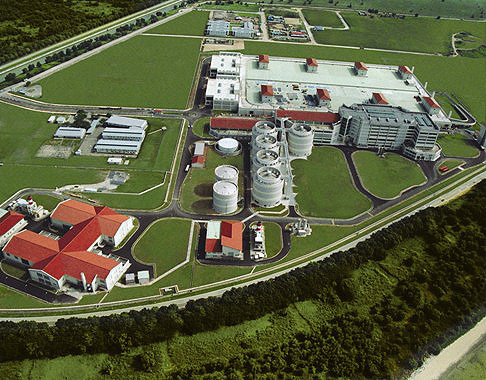
\includegraphics[width=0.42\textwidth]{changiwrp.jpg}
	\end{center}
	\caption[A centralized wastewater treatment plant in Singapore.]{A centralized wastewater treatment plant in Singapore. It has a wastewater treatment capacity of 800,000 m$^3/$day. \citep{changiwrp}} 
	\label{fig:changi}
\end{wrapfigure}%
In this project, we will focus on the wastewater management infrastructure of a city. As with other infrastructures described earlier, the wastewater treatment network in most cities today are centralized. Such treatment systems collect wastewater from households and are designed to handle large amounts of wastewater at a central location of the area it serves. With the implementation of centralized treatment systems in many countries, water pollution in those locations have been successfully controlled \citep{li2014}. In the past few decades, there has been a paradigm shift in the approach to water management. It is moving towards a stronger focus on how to best allocate water for human needs \citep{gleick2000}.

Typically, after treating the wastewater, centralized treatment systems redistribute the water back to the region for reuse or dispose the water into a water body. Additionally, centralized treatment systems require technology that are expensive, such as membrane bioreactors. 

\begin{wrapfigure}{R}{0.45\textwidth}
	\begin{center}
		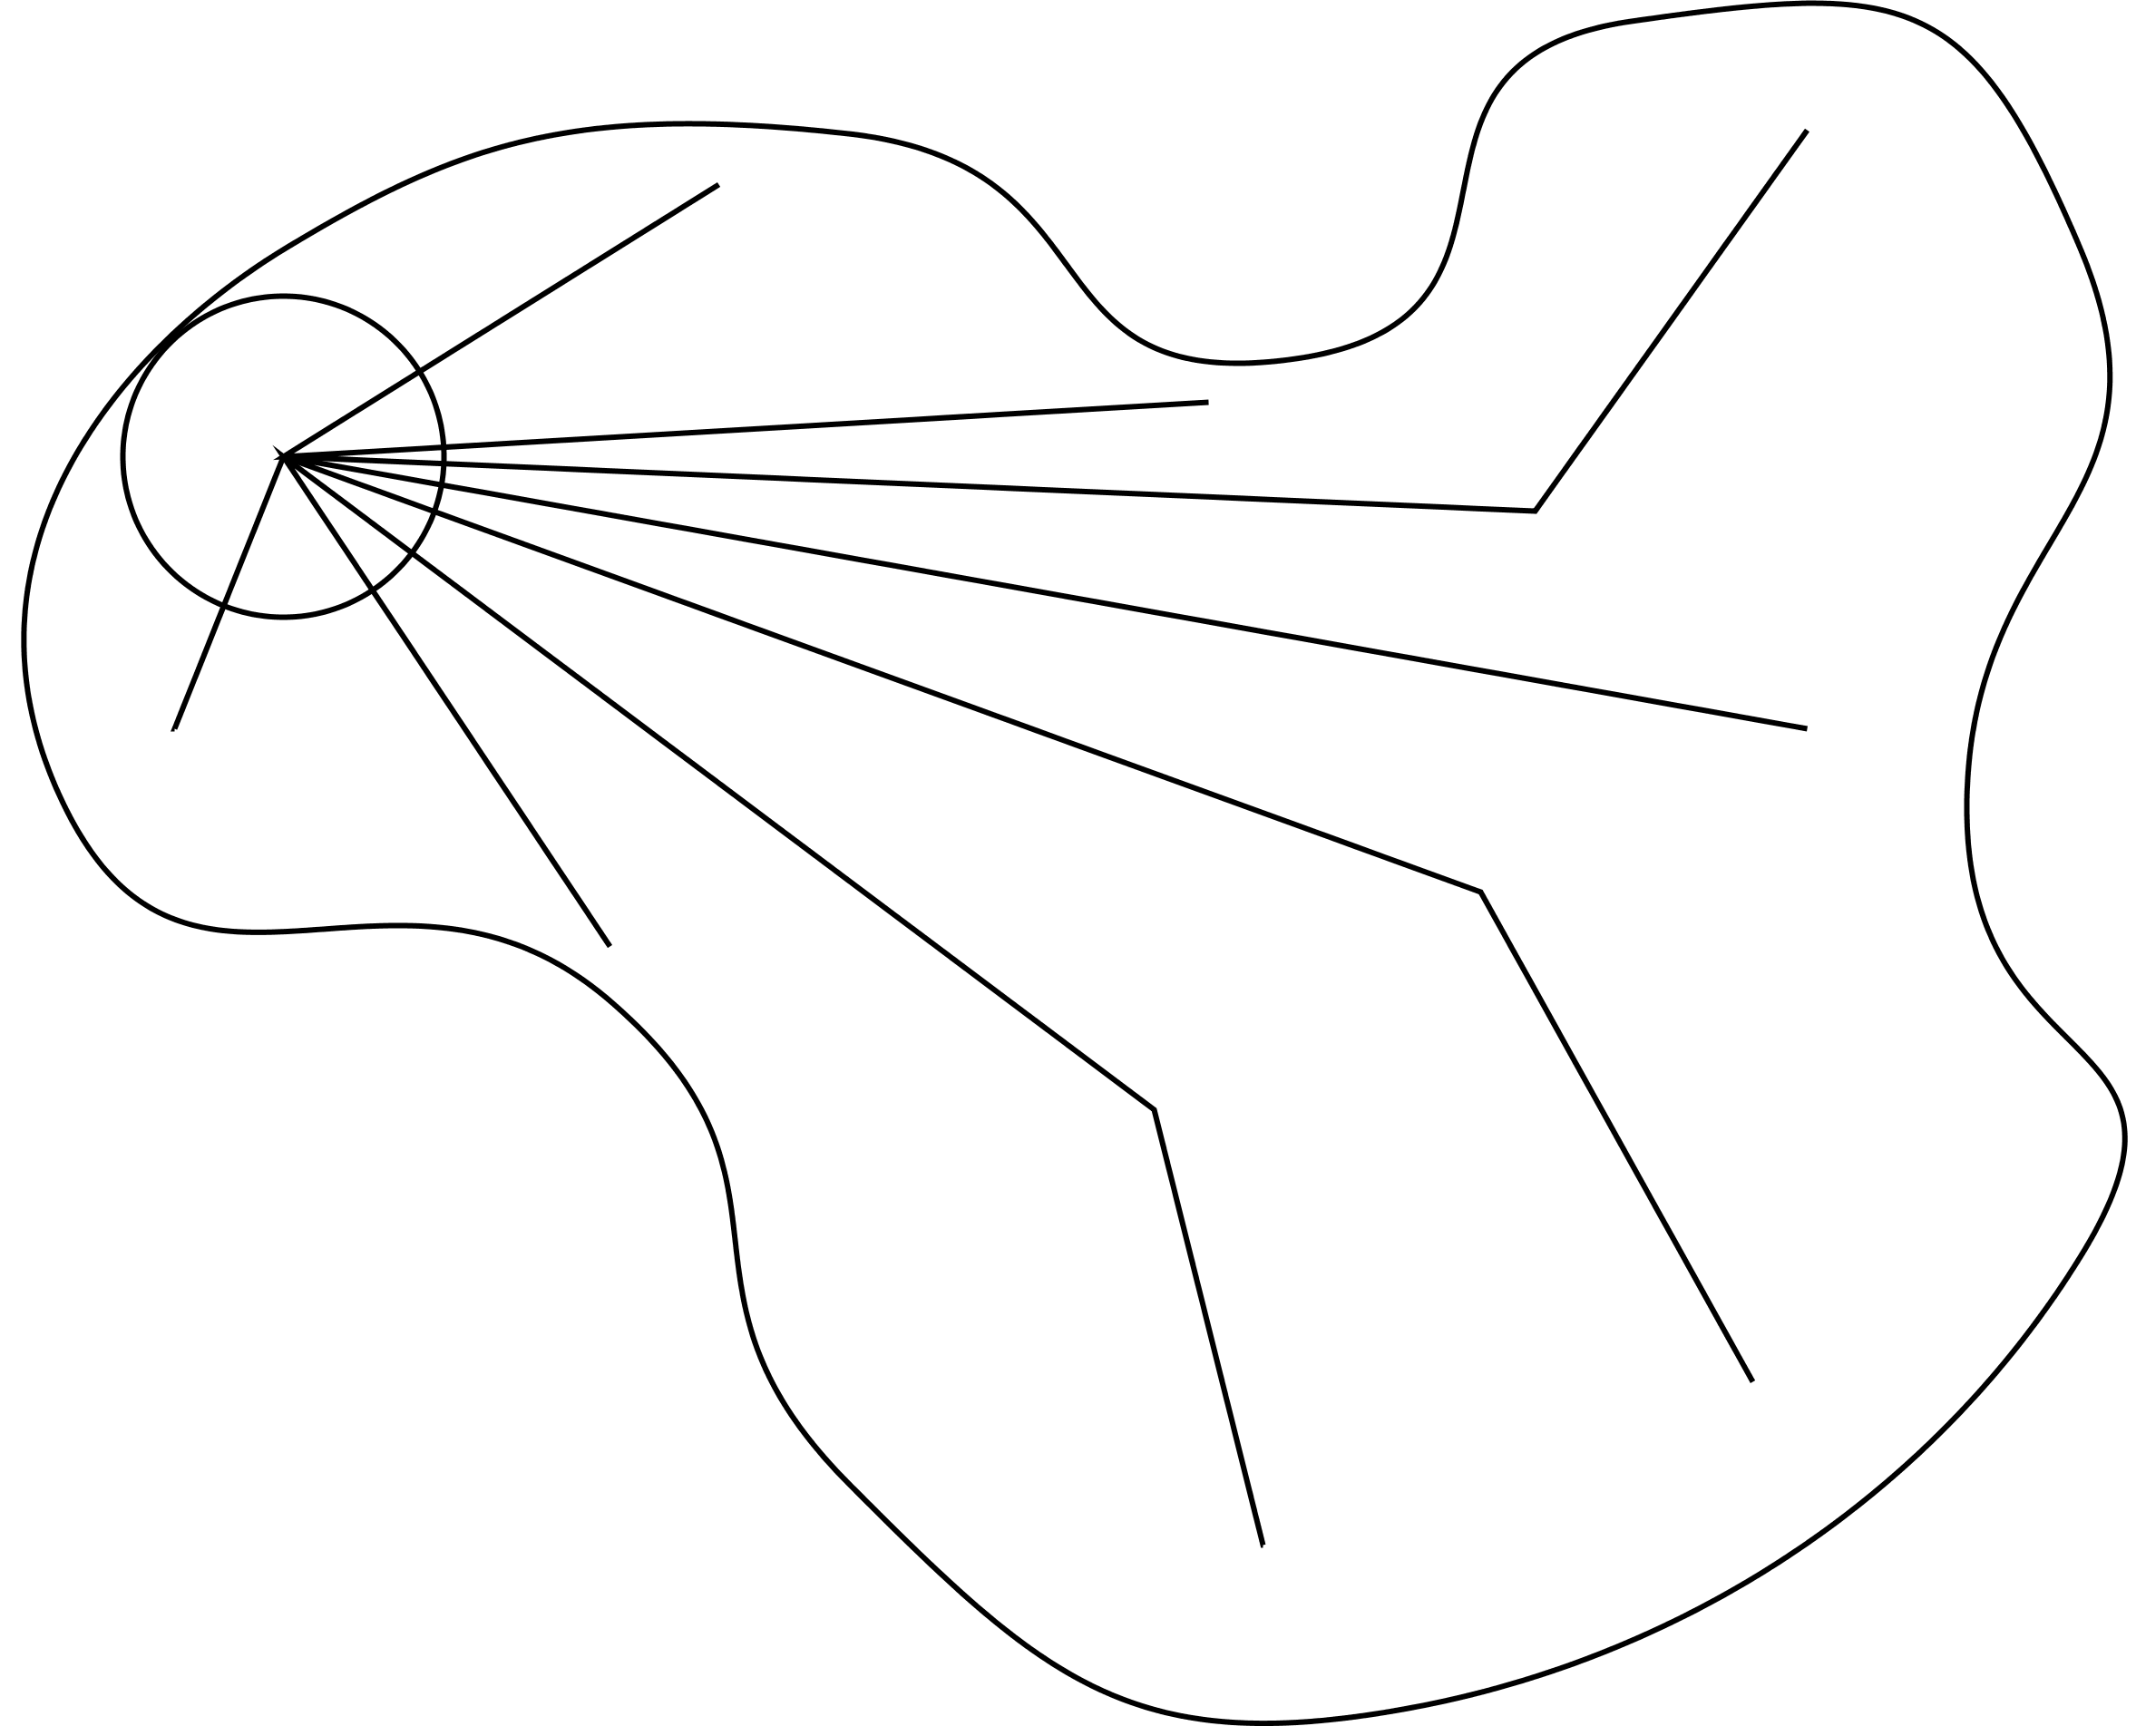
\includegraphics[width=0.42\textwidth]{centralizedtreatment.png}
	\end{center}
		\caption{A centralized wastewater treatment network.}
		\label{fig:cennet}
\end{wrapfigure}%
As urbanised areas grow in size and population, the amount of wastewater produced per day in an urban area increases. Hence, it is important to consider the water allocation and reuse within a region as it is costlier to bring water in from new sources \citep{gleick2000}. In addition to the negative consequences of relying on a single location for wastewater treatment \citep{wilderer2000,bakir2001}, a centralised wastewater management system itself becomes unwieldy and costly to build on a large scale \citep{wilderer2000}.


\begin{wrapfigure}{R}{0.45\textwidth}
	\begin{center}
		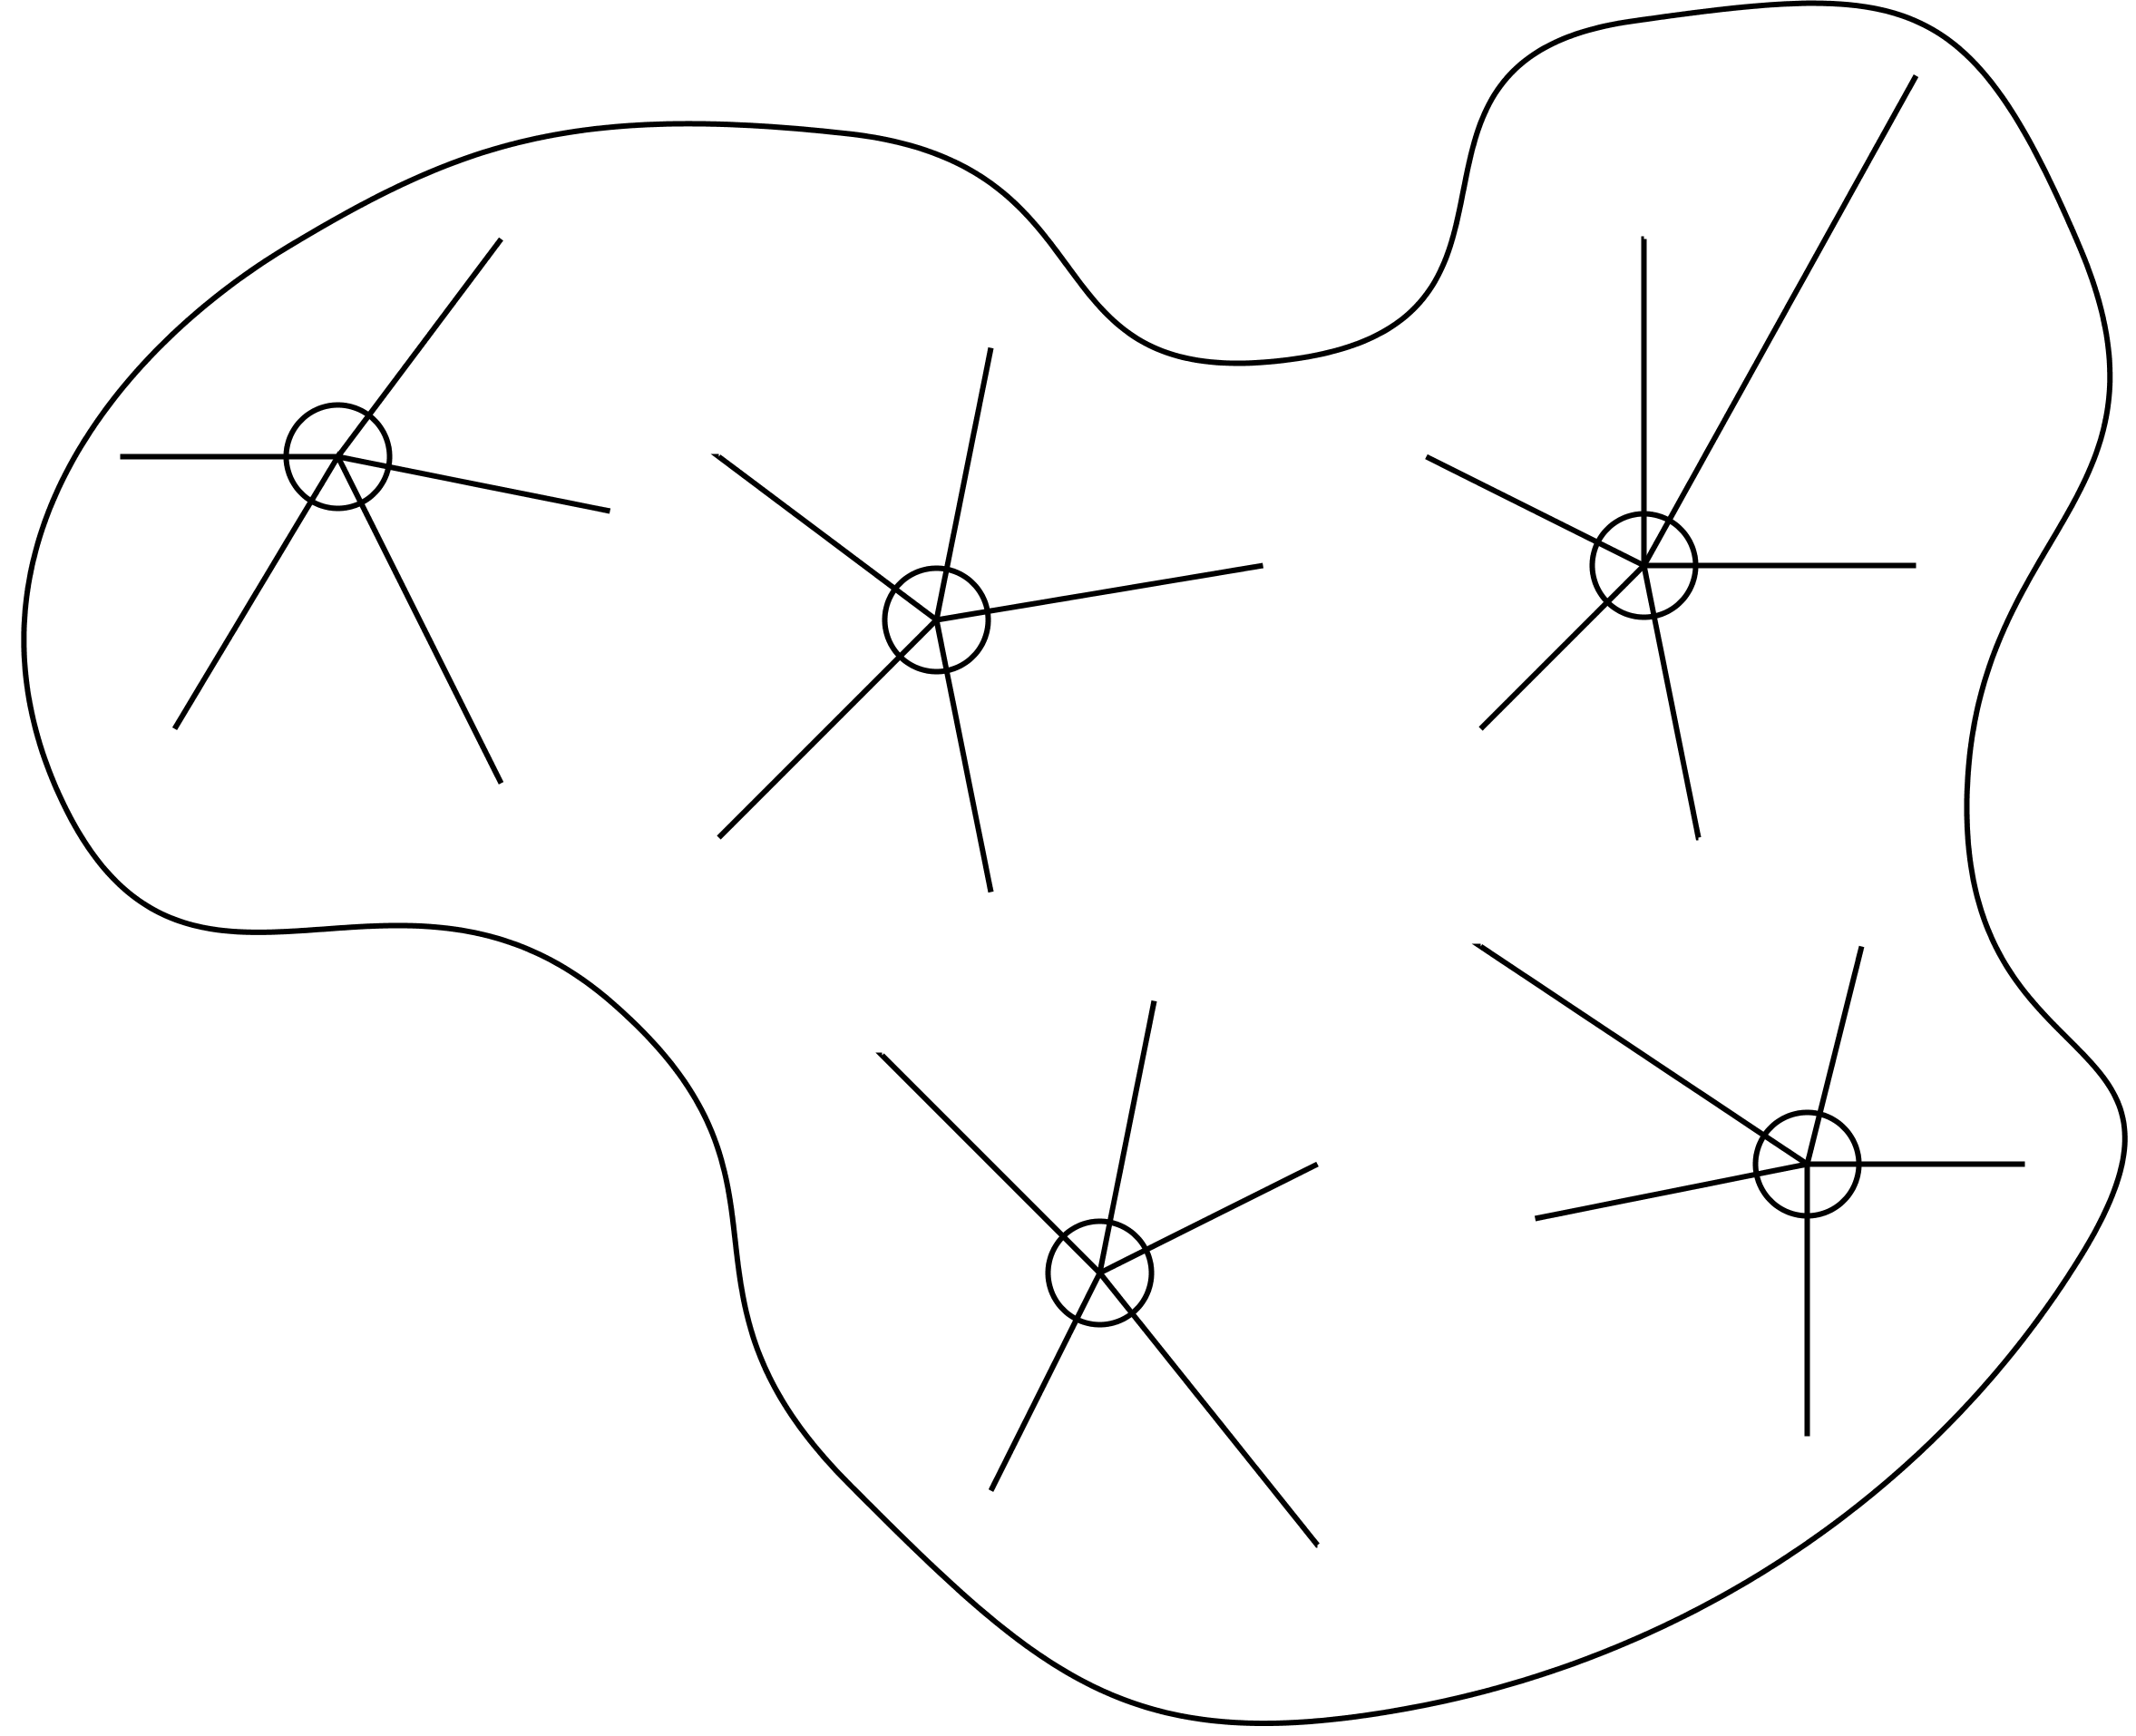
\includegraphics[width=0.42\textwidth]{decentralizedtreatment.png}
	\end{center}
		\caption{A decentralized wastewater treatment network.}
		\label{fig:decennet}
\end{wrapfigure}
In order to tackle this, decentralized wastewater management systems as in \autoref{fig:decennet} have been proposed to reduce the distance from the wastewater source to the release point, cutting down on the cost of transporting wastewater to a dedicated facility \citep{otterpohl1997,wilderer2000,bakir2001}. A decentralized wastewater treatment network approach encourages wastewater to be treated near to the source for reuse in the same area. To serve an area of the same size as a centralized wastewater system, a decentralized wastewater treatment system needs to have a larger quantity of plants with smaller scale operations. Various case studies have conducted a cost-benefit analysis on the implementation of a centralised wastewater management system against a decentralised one and have concluded that the decentralised wastewater management is generally cheaper to maintain \citep{prihandrijanti2008,mawss2015}. 



%\begin{figure}
%	\centering
%	\subfloat[A centralized wastewater treatment network.\label{subfig:cen}]{ %[t]{0.5\textwidth}
%		\includegraphics[width=0.42\textwidth]{centralizedtreatment}
%	}
%%		\caption{A centralized wastewater treatment network.}
%%		\label{fig:cennet}
%%	\end{subfigure}
%	\hfill
%	\subfloat[A decentralized wastewater treatment network.\label{subfig:decen}]{ %[t]{0.5\textwidth}
%		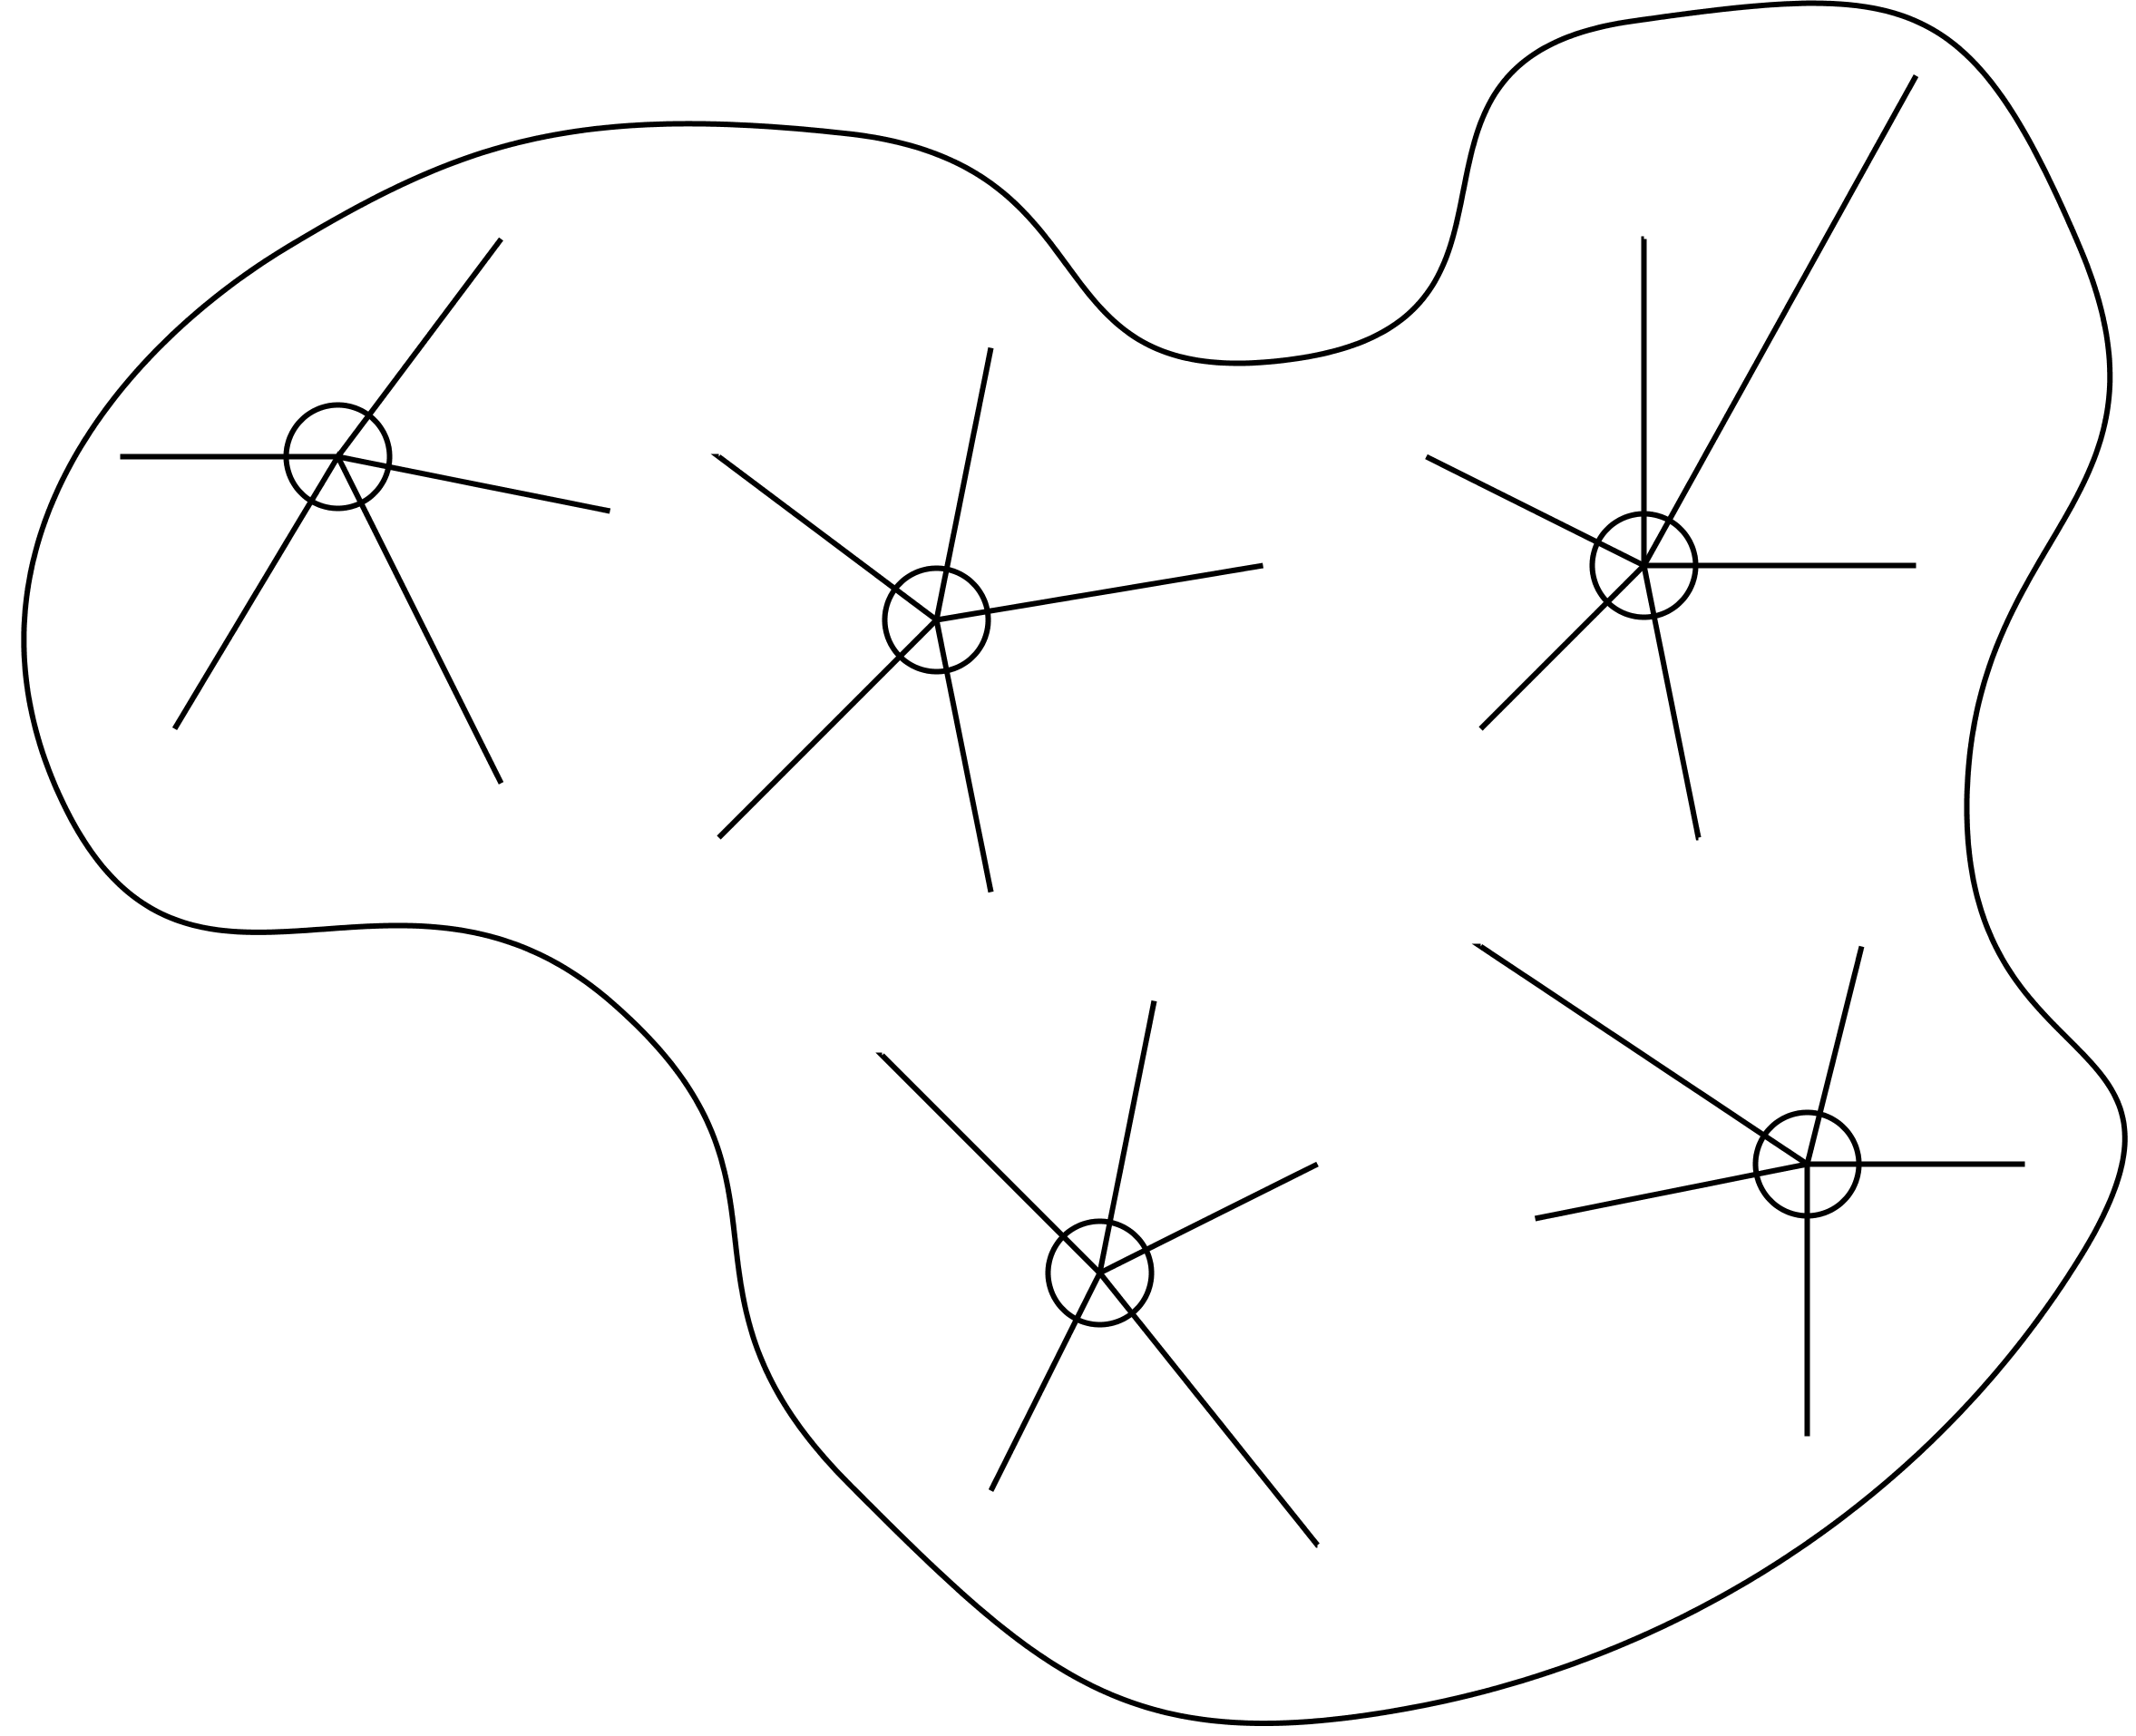
\includegraphics[width=0.42\textwidth]{decentralizedtreatment}
%	}
%%		\caption{A decentralized wastewater treatment network.}
%%		\label{fig:decennet}
%%	\end{subfigure}
%	\caption[Wastewater treatment networks.]{Wastewater treatment networks.} 
%	\label{fig:networks}
%\end{figure}

%  This removes the need to transport wastewater over large distances and meets the same goal.

\subsection{Decentralized wastewater management}
%Decentralized wastewater management systems such as constructed wetlands are increasingly gaining traction as the costs of construction become comparable to centralized wastewater management systems. 
There are many advantages decentralized systems give over centralized ones. For one, a decentralized system has more treatment sites, which reduces the impact of the failure of a single treatment site. If a centralized treatment plant were to fail, the wastewater collected will accumulate and there is no backup plant nearby available to treat the water. On the other hand, if one treatment site of a decentralized system fails, the wastewater may be rerouted to other sites temporarily, ensuring that the system does not come to a standstill. 

\subsection{Constructed Wetlands}
One approach to decentralised wastewater management is the constructed wetlands concept. Essentially, constructed wetlands aim to simulate real wetlands where water flows through and has its nutrients removed via biological processes. In the constructed version, wastewater flows through the wetland to provide the pollutants within as a nutrient source for plant absorption. The end product of wastewater going through these processes is water that meets the standards for release. The use of plants to treat the water allows the procedure of treating wastewater to be more hands off, thus requiring less maintenance. Thus, the costs involved in implementing constructed wetlands is relatively low as it uses the natural ability of plants to treat wastewater \citep{kadlec2009,mawss2015}. However, the cost effectiveness of constructed wetlands is contingent on the following: 
\begin{itemize}
	\setlength{\itemsep}{0pt}
	\setlength{\parskip}{0pt}
	\setlength{\parsep}{0pt}
	\item[-] Treatment sites are in optimal locations. 
	\item[-] Treatment sites are of a suitable size to handle the expected wastewater volume from the sources. 
\end{itemize}
The size of the constructed treatment wetlands has to be big enough to serve the amount of wastewater produced, but not too big as the system may collapse due to a lack of nutrients for the plants towards the end of the wetlands. Additionally, the location of the constructed wetlands has to be taken into consideration to determine the shortest distance of pipes required to link the wastewater sources to the treatment area to balance the cost of transporting wastewater and building the site. \citep{mawss2015} In order to determine the ideal location and size of constructed wetlands in a defined area, a mathematical model has been developed to represent the problem. Solving this model will give the ideal location and size of constructed wetlands to be designed.

\subsubsection{Horizontal sub-surface flow constructed wetlands}
\begin{wrapfigure}{R}{0.45\textwidth}
	\begin{center}
		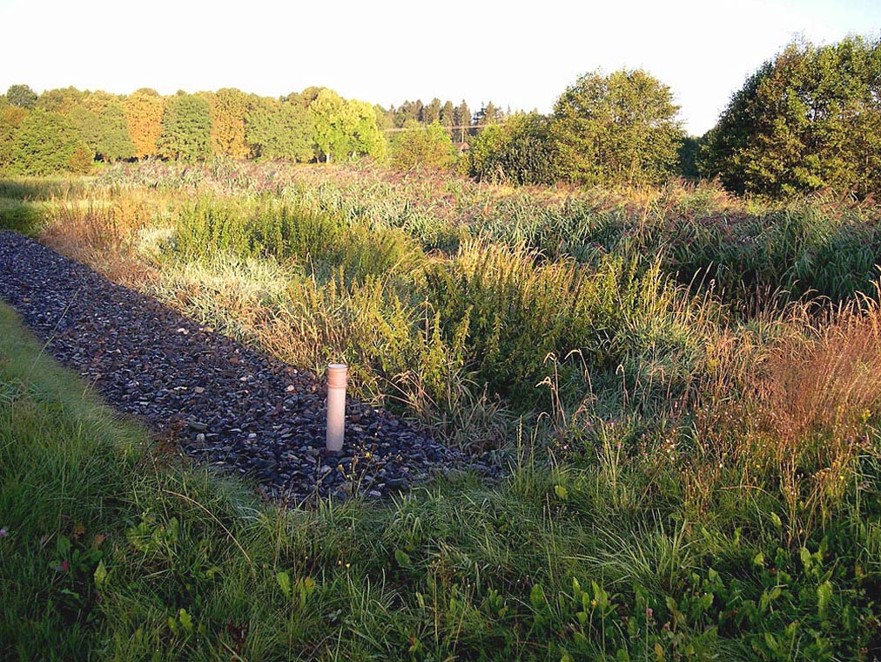
\includegraphics[width=0.42\textwidth]{hssf.jpg}
	\end{center}
	\caption[A horizontal sub-surface flow constructed wetlands in Czech Republic.]{A horizontal sub-surface flow constructed wetlands in Czech Republic. \citep{vymazal2008}} 
	\label{fig:changi}
\end{wrapfigure}
Over the years, implementation of more treatment wetlands in addition to higher water quality standards have encouraged studies to focus on establishing process design tools for the wetlands. Of all the types of wetlands that have been implemented, the horizontal sub-surface flow (HSSF) constructed wetlands is one of the most common. %\cite{rousseau2004model} recommends the first-order $k$-$C^*$ model for representing the constructed wetlands reaction process as it is a good balance between scientific accuracy and complexity as compared to other models that have been developed. 

\subsection{Objective}
%aim
While constructed wetlands can essentially be implemented wherever there is space, the maximum effectiveness of using this decentralized wastewater treatment system is only achieved when it is located at an optimal distance to the areas which it serves. The performance of constructed wetlands also depends on whether the size is sufficient to handle the projected wastewater flow rate from the area. In addition, the components of wastewater is easily affected by the source and weather. Due to this natural variation, the pollutant composition in wastewater is not deterministic. The ideal configuration (location and size) of treatment sites from a deterministic optimization model may not perform well under such uncertainty. Hence, this project aims to show how a stochastic model may be used in this situation to improve overall performance of the network with the application of the formulated model in an area in Mobile, Alabama. 

\subsection{Significance}
%of the project

\section{Methodology}\label{section:method}
\subsection{Case study: a decentralized CWs system for municipal wastewater treatment}
A case study approach is used to showcase the practical application of an optimization model for decentralized CW network to a real-life scenario. In this report, a case study of the optimal location and design size of a constructed wetlands treatment network in Mobile, Alabama.

\subsubsection{Mobile, Alabama}
With 412,992 people, Mobile County is the second most populated county within Alabama, a state in the United States. The population of Mobile County has been steadily increasing \citep{uscb2002census}. As populations grow, several fringe communities are created. In order to manage the wastewater produced by such communities, the traditional approach is to link these fringe communities up with long length large diameter pipes to transport all the wastewater produced to a single municipal wastewater treatment plant to be processed and then released into nearby water sources. In Mobile, the Mobile Area Water \& Sewer System (MAWSS) serves such fringe communities and overall serves approximately 530 square kilometres in Mobile County \citep{mawss2015}. MAWSS supports the region mostly through centralised wastewater treatment facilities. However, annual operations and maintenance costs for such centralised wastewater management systems have been shown to be costlier than decentralized ones. This is because decentralized treatment systems largely reduce the transport cost incurred and processes wastewater to be released very close to the community \citep{mawss2015}. Thus, implementation of decentralized wastewater management systems such as constructed wetlands are being considered to reduce expenses in the long term. 

Within Mobile, the constructed wetlands concept has been tested since 1997. \cite{surrency1997} designed and built a CW for urban stormwater management. His report recommended the implementation of constructed wetlands to replace wet ponds in managing stormwater. In 2005, MAWSS implemented a HSSF CW in Tricentennial Park in Mobile City as a trial to study the effectiveness of decentralized wastewater management systems in large urban sewer systems \cite{mawss2005}.
%talk about current implementations

%link to mawss experience with decentralization
%their problems faced?
%add to fast growing areas of cities without having to introduce new sewer lines
\subsubsection{Case Study Area}
\begin{wrapfigure}{R}{0.45\textwidth}%[!htb]
	\centering
	\includegraphics[width=0.35\textwidth]{blocks.png}
	\caption{Case study area in Mobile, Alabama.}
	\label{fig:blocks}
\end{wrapfigure}

The site chosen for the case study is near Mobile Regional Airport. It is a suburban area, mostly consisting of residences. As the objective of the project is to show how the optimization model can be applied, we have chosen a smaller area to keep the computation resources required reasonable. 

\section{Problem formulation}\label{section:problem}
\subsection{Qualitative model description}

\begin{figure}[!htpb]
	\centering
	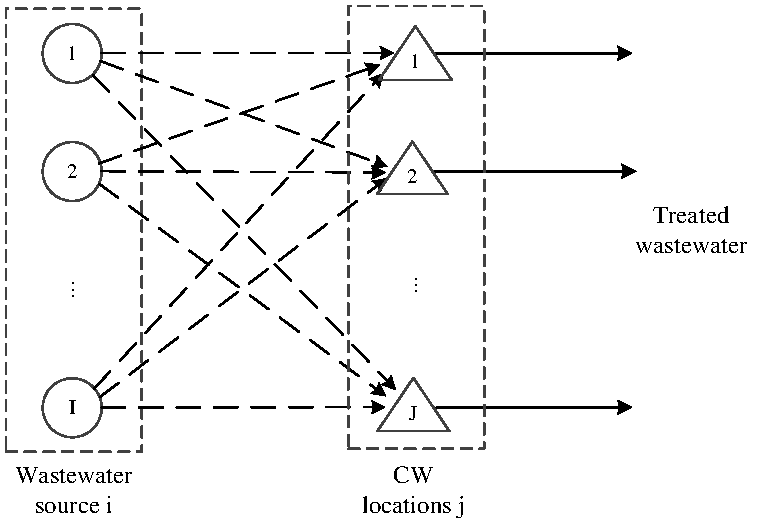
\includegraphics[width=0.7\textwidth]{CWnetwork.pdf}
	\caption{Superstructure of a decentralized CW treatment system network}
	\label{fig:network}
\end{figure}

In general, a decentralized constructed wetlands system in a region can be represented as in \autoref{fig:network}. Wastewater is generated from the sources $I$ and routed to constructed wetlands, where it is treated and discharged or reused on site. Thus, given a set of wastewater sources $I$ and a set of potential constructed wetlands locations $J$, the ultimate objective is to determine how to link the sources to the constructed wetlands, where the wetlands should be located and the size of the wetlands at the site. 

Besides this, in line with regulatory standards for treated water effluent, treatment targets are imposed on a set of pollutants $M$. This means that treated water leaving the constructed wetlands must have pollutant concentrations below specified levels. Depending on the intended use for treated water, treatment targets may be adjusted accordingly for each constructed wetlands site. This constraint directly affects the size of the constructed wetlands for a site as the size of the site determines the pollutant removal rate. It also indirectly affects the routing of the wastewater sources to the treatment sites. 

Thus, a solution is deemed feasible only when it satisfies all the constraints. However, due to natural variation in the environment and pollutant concentration of the influent wastewater, constructed wetlands may not always effectively remove pollutants. In reality, it is also unlikely that the treated wastewater meets the targets all the time. 

Additionally, cost is a major factor for decision makers to take into account hence the best feasible solution should be one that incurs the least cost. The cost consideration affects how the wastewater sources are routed to the treatment sites as the longer the distance, the higher the cost of constructing the pipe to link the source and site up. For the model, the following assumptions are made:
%explain why operational costs are not going to be considered

\begin{itemize}
	\setlength{\itemsep}{0pt}
	\setlength{\parskip}{0pt}
	\setlength{\parsep}{0pt}
	\item[-] wastewater from each source $i=1,...,I$ can be allocated to multiple constructed wetlands sites and each constructed wetlands can also treat wastewater from multiple wastewater sources. Sewer lines are needed to be constructed between wastewater sources and constructed wetlands. 
	\item[-] for any location $j=1,...,J$, if it is determined to construct a constructed wetlands, $K$ design options $k=1,...,K$ could be selected. Otherwise, we use $k=0$ to indicate that this location is not chosen to construct any constructed wetlands. 
	\item[-] a list of $M$ pollutants $m=1,...,M$ are evaluated. Treatment target $\tau_j^m$ is set for each pollutant $m$ and each potential site $j$.
\end{itemize}

\subsection{Deterministic model}\label{detmodel}

A basic list of model parameters and decision variables is provided in \autoref{table:modelparameter}. Other notations would be introduced and defined as per required in the rest of the paper. Before the uncertainty component is addressed, we will consider a model where there are no stochastic components.

\begin{table}[!htb]
	\setlength{\extrarowheight}{1.5mm}
	\caption{Notations of model parameters and decision variables}
	\begin{tabular}{|p{1.5cm} p{16cm}|}
		\hline
		\multicolumn{2}{|c|}{Indices} \\
		\hline
		$i$ & index of wastewater sources, $i\in\{1,2,...,I\}$\\
		$j$ & index of potential CW locations, $j\in\{1,2,...,J\}$ \\
		$m$ & index of evaluated water pollutants, $m\in\{1,2,...,M\}$\\
		$k$ & index of CW construction options, $k\in\{0,1,2,...,K\}$\\
		\hline
		\multicolumn{2}{|c|}{Model parameters} \\
		\hline
		$\varepsilon_i^m$ & concentration of pollutant $m$ in the wastewater source $i$ (mg/m$^3$)\\
%		$\varepsilon_{in,j}^m$ & concentration of pollutant $m$ in the influent of CW site $j$ (mg/m$^3$)\\
%		$\varepsilon_{out,j}^m$ & concentration of pollutant $m$ in the effluent of CW site $j$ (mg/m$^3$)\\
		$\tau_{j}^m$ & treatment target above background concentration for pollutant $m$ in CW site $j$ (mg/m$^3$)\\
		$F_{i}$ & total wastewater flow generated by source $i$ (m$^3$/d)\\
		$Q_{jk}$ &  flow capacity of CW in option $k$ for site $j$ (m$^3$/d)\\
		$A_{jk}$ & area of CW in option $k$ for site $j$ (m$^2$)\\		
		$c_{cw,jk}$ & construction cost of CW in design option $k$ for site $j$ (\$) \\	
		$d_{ij}$ & distance between wastewater source $i$ and site $j$ (m)\\
		$c_s$ & unit construction cost of sewer lines per distance (\$/m)\\
		\hline
		\multicolumn{2}{|c|}{Decision variables}\\
		\hline	
		$x_{ij}$ & binary variable, $x_{ij}=1$ if sewer lines are constructed from wastewater source $i$ to CW site $j$ and $0$ otherwise\\
		$y_{jk}$ & binary variable, $y_{jk}=1$ if construction option $k$ is chosen for site $j$ and $0$ otherwise. In particular, $y_{j0}$ denotes the choice of not constructing any CWs in site $j$\\
		$z_{ij}$ & volume of wastewater flow assigned from wastewater source $i$ to the CW in site $j$ (m$^3$)\\
		\hline	
	\end{tabular}

	\label{table:modelparameter}
\end{table}

\renewcommand{\theequation}{\thesection--\arabic{equation}}
\subsubsection{Objective Function}
For the deterministic case, the objective of the problem is to minimize the total cost of implementing the system in a region. 
\begin{align}
	&min \sum_{i=1}^I \sum_{j=1}^J d_{ij} c_s x_{ij} + \sum_{j=1}^J \sum_{k=1}^K c_{cw,jk} y_{jk}
\end{align}

\subsubsection{Constraints}
The following constraints formulate the constructed wetlands design option, wastewater allocation between sources and constructed wetlands, pollutant removal performance and treatment target fulfillment:


\noindent\textbf{Pollutant removal performance and treatment target fulfillment} 

First, we consider the influent of the constructed wetlands. The water that is entering the constructed wetlands should have the same amount of pollutants as all of the sources that are contributing wastewater to the site. So, the concentration of pollutant $m$ in the influent at each potential CW site, $\varepsilon_{in,j}^m$ can be determined with \autoref{eqn:influentformula}.
\begin{align} \label{eqn:influentformula}
	&\varepsilon_{in,j}^m = \frac{\varepsilon_i^m \sum_{i=1}^I z_{ij}}{\sum_{i=1}^I z_{ij}} && \forall j
\end{align}

To determine the pollutant concentration in the effluent, $\varepsilon_{out,j}^m$, we use a first-order $k-C^*$ model \citep{rousseau2004model} to calculate the pollutant removal. The $k-C^*$ model uses a plug-flow reactor model to represent the reactions during the pollutant removal process as depicted in \autoref{fig:plugflow}. The treatment rate of a pollutant $m$ in a HSSF CW with design option $k$ at site $j$ can be represented with a first-order $k-C^*$ model in the following equation:
\begin{align}
	\label{eqn:plugflow}
	&\varepsilon_{out,j}^m - C_j^{m*} = e^{-\frac{A_{jk}}{Q_{jk}}k_A^m} [\varepsilon_{in,j}^m - C_j^{m*}] && \forall j,k,m
\end{align}
where $k_A^m$ is the areal rate constant for pollutant $m$.

\begin{figure}[!htpb]
	\centering
	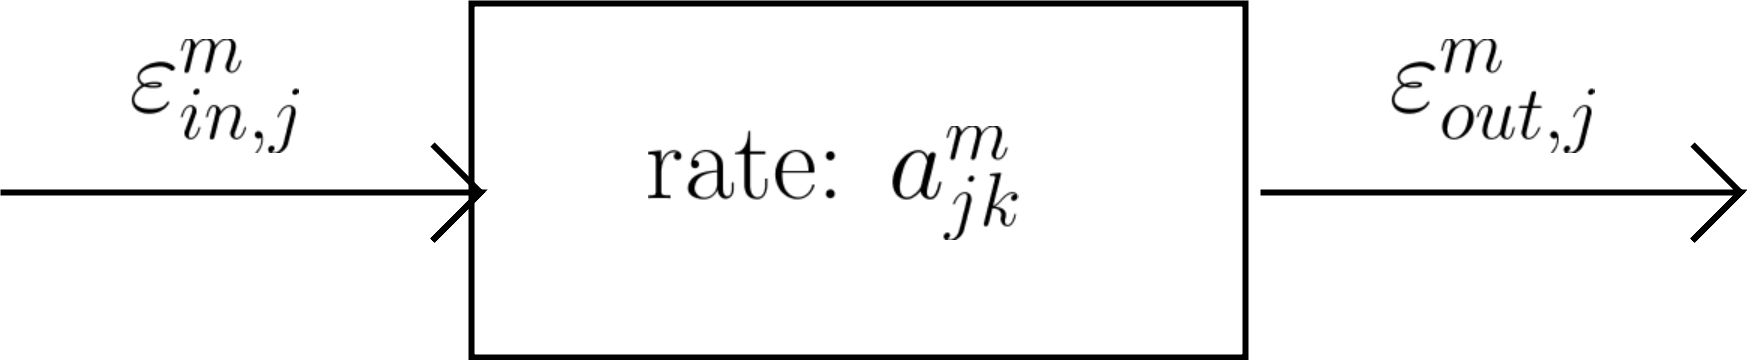
\includegraphics[width=0.5\textwidth]{plugflow.png}
	\caption{Pollutant treatment process}
	\label{fig:plugflow}
\end{figure}

The areal rate constant $k_A^m$ is determined empirically for each pollutant and varies depending on the region that the data is collected from. For the purposes of the case study, we will be using $k_A^m$ values based on data from North America as collated by \cite{vymazal2008}. 

As the area $A_{jk}$ and flow capacity $Q_{jk}$ of the CWs are determined beforehand with the various design options, expansion of the right hand side of \autoref{eqn:plugflow} shows that the effluent pollutant concentration is a linear function of the influent pollutant concentration that follows the expression $ax+b$. To simplify the linear program definition, the following parameters will be used in place of the full form of the coefficient: 
\begin{align}
	&a_{jk}^m = e^{-\frac{A_{jk}}{Q_{jk}}k_A^m} &&\forall j,k,m\nonumber\\
	&b_{jk}^m = C^* e^{-\frac{A_{jk}}{Q_{jk}}k_A^m} &&\forall j,k,m\nonumber\\
	&\varepsilon_{out,j}^m - C_j^{m*} = a_{jk}^m \varepsilon_{in,j}^m + b_{jk}^m && \forall j,k,m \label{eqn:newplugflow}
\end{align}

With the simplified parameters, \autoref{eqn:plugflow} can now be represented with \autoref{eqn:newplugflow}. After the wastewater is treated, the effluent is expected to meet pollutant concentration targets, $\tau_j^m$. Since the treatment targets are set at a value above the background concentration, the constraint will be as follows:
\begin{align}
	&\varepsilon_{out,j}^m - C_j^{m*} \leq \tau_j^m && \forall j,m \label{eqn:target}
\end{align}

Combining Equations \ref{eqn:influentformula}, \ref{eqn:newplugflow} and \ref{eqn:target}, we will have a constraint that ensures the effluent pollutant concentration is under the treatment target. The nonlinearity in the constraint was resolved by introducing a Big M. In our model, the Big M is calculated using the %fill in
\begin{align}
	&\sum_{i=1}^{I} (a_{jk}^m \varepsilon_i^m + b_{jk}^m) z_{ij} - M_1(1 - y_{jk}) \leq \tau_j^m \sum_{i=1}^I z_{ij}  && \forall j,k,m
\end{align}
\\
\noindent\textbf{Wastewater allocation from sources to sites} 

Let $x_{ij}$ be a binary variable that describes the interconnection between the wastewater source $i$ and potential contructed wetlands site $j$. When $x_{ij} = 1$, there is a pipe constructed between wastewater source $i$ and potential constructed wetlands site $j$. Wastewater is allowed to flow from source $i$ to site $j$. Otherwise, when $x_{ij} = 0$, there is no pipe connecting wastewater source $i$ and potential constructed wetlands site $j$. 

All the wastewater produced in the region studied has to be treated, so there should not be any excess wastewater volume. On top of that, the total volume of wastewater flowing into a constructed wetland cannot exceed the design capacity of the constructed wetland. If $y_{j0} = 1$ for any $j$, there should not be any pipes connecting any wastewater source $i$ to the respective potential constructed wetlands site $j$. Finally, there should only be wastewater sent to a site $j$ if the wastewater source $i$ and potential constructed wetlands site $j$ is connected (i.e. $x_{ij} = 1$). 

If $z_{ij}$ represents the volume of wastewater sent from source $i$ to site $j$, $F_{i}$ is the total wastewater flow from source $i$ and $Q_{jk}$ is the maximum flow capacity accepted by site $j$ with design option $k$:
\begin{align}
	&\sum_{i=1}^{I}z_{ij}\leq \sum_{k=0}^{K}Q_{jk}y_{jk},~~ &&\forall j\\
	&\sum_{j=1}^J z_{ij} = F_i,&&\forall i\\
	&x_{ij} + y_{j0} \leq 1 && \forall i,j \\
	&x_{ij}\in\{0,1\}&&\forall i,j\\
	&z_{ij} \geq 0 && \forall i,j %\nonumber
\end{align}

\noindent\textbf{Constructed wetlands design options} 

Let $y_{jk}$ be a binary variable that describes the design option $k$ selected for the constructed wetlands site $j$. In the case where $k=0$, there will be no constructed wetlands on the potential site $j$. Otherwise, any other values for $k$ will correspond to the respective design options available. When $y_{jk} = 1$, it means that there will be a constructed wetlands of type $k$ at site $j$. 

The different design options result in different construction costs and pollutant removal capacities. At each potential CW site, there can only be one design option selected. Hence, the following constraints are introduced:
\begin{align}
	%\begin{split}
	&\sum_{k=0}^{K}y_{jk}=1&&\forall j\\
	&y_{jk}\in\{0,1\}&&\forall j,k
	%\end{split}
\end{align}
 
%		$a_{jk}^m$ & areal rate constant coefficient for option $k$ at site $j$ for pollutant $m$\\
%		$b_{jk}^m$ & background areal rate constant for option $k$ at site $j$ for pollutant $m$\\
%\begin{alignat*}{2}
%	&{\sum_{i=1}^{I}F_{i}y_{ij}\varepsilon_{i}^{m}} = \varepsilon_{in,j}^{m}{\sum_{i=1}^{I}F_{i}y_{ij}} &&\forall j,m\\
%	&[\varepsilon_{in,j}^{m}-{c}_{j}^{m*}]\sum_{k=0}^{K}e^{-\frac{A_{jk}}{Q_{jk}}k_{A}^{m}}z_{jk}+c_{j}^{m*} = \varepsilon_{out,j}^{m} &&\forall j,m\\
%	&\varepsilon_{out,j}^{m}\leq \tau_{j}^{m}~~~&&\forall j\\
%	&a_{jk}^m = e^{-\frac{A_{jk}}{Q_{jk}}k_{A}^{m}}\\
%\end{alignat*}

\subsubsection{Model}
The following deterministic model is developed from the above constraints. It is a \emph{Mixed-Integer Linear Programming} (MILP) problem (Model D):
\setcounter{equation}{0}
\counterwithout{equation}{section}
%\begin{equation}\label{modelD}
%\begin{aligned}
\begin{align}\label{model:D}
	\text{Model D}:~~&min ~ \sum_{i=1}^{I}\sum_{j=1}^{J}d_{ij}c_s x_{ij} + \sum_{j=1}^{J}\sum_{k=1}^{K}c_{cw,jk}y_{jk}\nonumber\\~~
	\mbox{s.t.}~~
	&\sum_{i=1}^{I} (a_{jk}^m \varepsilon_i^m + b_{jk}^m) z_{ij} - M_1(1 - y_{jk}) \leq \tau_j^m \sum_{i=1}^I z_{ij}  && \forall j,k,m\\
 	&\sum_{i=1}^{I} z_{ij} \leq \sum_{k=0}^K Q_{jk} y_{jk} && \forall j\\
	&\sum_{j=1}^J z_{ij} = F_i && \forall i\\
	&z_{ij} \leq F_i x_{ij} && \forall i,j\\
	&x_{ij} + y_{j0} \leq 1 && \forall i,j\\
	&\sum_{k=0}^{K}y_{jk} = 1&&\forall j\\
	&x_{ij} \in \{0,1\}&&\forall i,j\\
	&y_{jk} \in \{0,1\}&&\forall j,k\\
	&z_{ij} \geq 0&&\forall i,j
\end{align}
%\end{aligned}
%\end{equation}
\renewcommand{\theequation}{\thesection--\arabic{equation}}
\setcounter{equation}{13}
\subsection{Two-stage stochastic model}\label{stomodel}
%-	Justify why stochastic needs to be considered
%-	Why we are only going to use one stochastic variable
%-	How to extend deterministic to the stochastic model? 
In a real situation, the pollutant loading of wastewater is uncertain as they fluctuate depending on the actual weather, activities carried out for the day (laundry, showers, etc.) and other reasons. With this uncertainty, the CW network in the optimal solution for the deterministic model may not be able to perform well over a long period of time. If we take the uncertainty into consideration in the model before solving it, we may be able to attain a better optimal solution that is expected to meet the treatment standards more frequently. 

We will use a two-stage stochastic model to incorporate the uncertainty into the model. The first-stage variables will be the construction options of the potential CW sites, $y_{jk}$ and the connections between the wastewater sources and the potential CW sites, $x_{ij}$. The second-stage variable will be the volume of wastewater to be sent from the wastewater sources to the potential CW sites. In this section, the variable will be denoted as $z_{ij} (\tilde{\varepsilon})$ to show that it is dependent on the influent pollutant concentration. As we are considering a long run average, we will keep the total wastewater volume per day produced by each wastewater source $i$ constant. 
%insert stochastic model

\subsubsection{Objective function}
In the stochastic model, we want to ensure that the best possible performance of the CW network is attained. Thus, the objective function will be to maximize the probability of the effluent pollutant concentrations meeting the treatment standards. 
\begin{align}
	&max~\bP(\tilde{\varepsilon}_{out} \leq \tau)
\end{align}

\subsubsection{Constraints}
Most of the constraints in the model are the same as the ones in Model D for wastewater allocation and the constructed wetlands design options. Since the pollutant treatment performance is evaluated in the objective function, the constraints are left in their original nonlinear expressions for now. 

\noindent\textbf{Cost}

As the objective function is no longer to minimize the cost, a new constraint will be used to take the budget concerns into account. In this case, we will set the budget to be 5\% above the total cost of the optimal solution from Model D (\autoref{constraint:budget}). Allowing the cost to go above the minimum found in the deterministic model gives some leeway for the model to achieve better pollutant treatment performance at a slightly higher cost.
\begin{align}\label{constraint:budget}
	&\sum_{i=1}^I \sum_{j=1}^J d_{ij} c_s x_{ij} + \sum_{j=1}^J \sum_{k=1}^K c_{cw,jk} y_{jk} \leq B 
\end{align}


\subsubsection{Model}
\setcounter{equation}{0}
\counterwithout{equation}{section}
The two-stage stochastic model of the problem (Model S) is described following the above modifications from Model D.
\begin{align}
	\text{Model S}:~~&max~\bP(\tilde{\varepsilon}_{out} \leq \tau) \nonumber\\~~
	\mbox{s.t.}~~
	&\tilde{\varepsilon}_{in,j}^m = \frac{\sum_{i=1}^I z_{ij}(\tilde{\varepsilon}) \tilde{\varepsilon}_i^m}{\sum_{i=1}^I z_{ij}(\tilde{\varepsilon})} && \forall j,m\label{constraint:inf}\\
	&\tilde{\varepsilon}_{out,j}^m - C_j^{m*} = [\tilde{\varepsilon}_{in,j} - C_j^{m*}] \sum_{k=1}^K a_{jk}^m y_{jk} && \forall j,m\label{constraint:eff}\\
	&\sum_{i=1}^I \sum_{j=1}^J d_{ij} c_s x_{ij} + \sum_{j=1}^J \sum_{k=1}^K c_{cw,jk} y_{jk} \leq B \\
	&\sum_{i=1}^I z_{ij} (\tilde{\varepsilon}) \leq \sum_{k=1}^K Q_{jk} y_{jk} && \forall j\\
	&\sum_{j=1}^J z_{ij} (\tilde{\varepsilon}) \leq F_i && \forall i\\
	&z_{ij} (\tilde{\varepsilon}) \leq F_i x_{ij} && \forall i,j\\
	&x_{ij} + y_{j0} \leq 1 && \forall i,j\\
	&\sum_{k=0}^K y_{jk} = 1 && \forall j \\
	&x_{ij} \in \{0, 1\} && \forall i,j\\
	&y_{jk} \in \{0, 1\} && \forall j,k\\
	&z_{ij}(\tilde{\varepsilon}) \geq 0 && i,j 
\end{align}
\renewcommand{\theequation}{\thesection--\arabic{equation}}
\subsection{Sample average approximation}
% two-stage  using SAA to estimate the probability
%two ways
% max avg success
% min avg shortfall
%
In order to evaluate the problem, the sample average approximation method will be used to form a deterministic equivalent of the stochastic model. Realizations of the uncertain parameter will replace the stochastic component. Each scenario to be evaluated will have a set of realizations of the concentration of each pollutant $m$ from each wastewater source $i$. Let $n$ represent a scenario to be evaluated ($n \in \{1,..,N\}$). The number of scenarios $N$ to be evaluated is set to 100. 

Estimating the probability of the effluent pollutant concentrations meeting the treatment targets can be done with two different methods. For the first method, each scenario is given a success variable  - a binary variable that takes the value 1 if the scenario is successful and 0 otherwise. Any scenario $n$ will be successful if the treatment target $\tau_j^m$ is met by all effluents and all pollutants. The objective function then aims to maximize the average of the success variable across all scenarios $N$. This method directly estimates the probability of the treatment target being met in the long run. Further elaboration on this method is in Section \ref{subsect:maxsuccess}. The second method measures the mass of pollutants in excess of the treatment target. Each scenario has a variable that will be set to the largest excess mass of all the effluents for each pollutant $m$. When all effluents in a scenario $n$ do not exceed any of the pollutant treatment targets $\tau_j^m$, the new variables are set to 0. The objective function in this method aims to minimize the average amount by which the effluents exceed treatment targets. Section \ref{subsect:minshortfall} covers this method in more detail.

\begin{table}[!htb]
	\setlength{\extrarowheight}{1.5mm}
	\caption{Notations of additional model parameters and decision variables}
	\begin{tabular}{|p{1.5cm} p{16cm}|}
		\hline
%		\multicolumn{2}{|c|}{Indices} \\
%		\hline
%		$n$ & index of scenarios to be generated, $n\in\{1,2,...,N\}$\\
%		\hline
		\multicolumn{2}{|c|}{Model parameters} \\
		\hline
		$\varepsilon_i^{mn}$ & concentration of pollutant $m$ in the wastewater source $i$ for scenario $n$ (mg/m$^3$)\\
%		$\varepsilon_{in,j}^m$ & concentration of pollutant $m$ in the influent of CW site $j$ (mg/m$^3$)\\
%		$\varepsilon_{out,j}^m$ & concentration of pollutant $m$ in the effluent of CW site $j$ (mg/m$^3$)\\
		\hline
		\multicolumn{2}{|c|}{Decision variables}\\
		\hline	
%		$x_{ij}$ & binary variable, $x_{ij}=1$ if sewer lines are constructed from wastewater source $i$ to CW site $j$ and $0$ otherwise\\
%		$y_{jk}$ & binary variable, $y_{jk}=1$ if construction option $k$ is chosen for site $j$ and $0$ otherwise. In partiular, $y_{j0}$ denotes the choice of not constructing any CWs in site $j$\\
		$z_{ij}^n$ & volume of wastewater flow assigned from wastewater source $i$ to the CW in site $j$ in scenario $n$  (m$^3$)\\
		$\gamma^n$ & binary variable, $\gamma^n = 1$ if all pollutants in all effluents $\varepsilon_{out,j}^mn$ for scenario $n$ meet the treatment target $\tau_j^m$\\
		$\lambda_{ijk}^n$ & variable for the McCormick envelope for the bilinear term $y_{jk}$ and $z_{ij}^n$\\ 
		\hline	
	\end{tabular}
	\label{table:modelparameterss1}
\end{table}

\subsubsection{Maximizing average success}\label{subsect:maxsuccess}
%explain formulation
As described in the previous section, the objective of this method is to maximize the average success of all scenarios $N$. New parameters and decision variables in this model are defined in \autoref{table:modelparameterss1}. This expanded model is defined in Model S1. The success variable $\gamma^n$ is combined together with the two pollutant treatment equations \ref{constraint:inf} and \ref{constraint:eff} in Model S. The resulting constraint has two nonlinear terms which is resolved using the Big M method as well as using McCormick envelopes to relax the problem. The form of the revised constraint is in \autoref{constraint:treatments1} of Model S1.

\setcounter{equation}{0}
\counterwithout{equation}{section}
\begin{align}%\label{model:S1}
%\begin{equation}\label{modelS1}
%\begin{aligned}
	\text{Model S1}:~~&max ~ \frac{1}{N}\sum_{n=1}^N \gamma^n \nonumber \\~~
	\mbox{s.t.}~~
	%gamma constraint
%	&\varepsilon_{out,j}^{mn} - \tau_j^m + M_1(\gamma^n - 1) \leq 0 && \forall j,m,n\\
	%pollutant treatment constraint (problematic)
%	&\sum_{i=1}^{I} (a_{jk}^m \varepsilon_i^{mn} - b_{jk}^m) z_{ij}^n - M_2(1 - y_{jk}) = \varepsilon_{out,j}^{mn} \sum_{i=1}^I z_{ij}^n  && \forall j,k,m,n\\
	&\sum_{k=1}^K \sum_{i=1}^I (a_{jk}^m \varepsilon_i^{mn} + b_{jk}^m) \lambda_{ijk}^n - \tau_j^m \sum_{i=1}^I z_{ij}^n \leq M_2 (1-\gamma^n) && \forall j,m,n \label{constraint:treatments1}\\	
	%cost constraint
	&\sum_{i=1}^{I}\sum_{j=1}^{J}d_{ij}c_s x_{ij} + \sum_{j=1}^{J}\sum_{k=1}^{K}c_{cw,jk}y_{jk} \leq B && \\
	%capacity constraint
 	&\sum_{i=1}^{I} z_{ij}^n \leq \sum_{k=0}^K Q_{jk} y_{jk} && \forall j,n\\
	%maximum flow from source
	&\sum_{j=1}^J z_{ij}^n = F_i && \forall i,n\\
	%send water only if connected
	&z_{ij}^n \leq F_i x_{ij} && \forall i,j,n\\
	%enforce no connection if there is no CW constructed
	&x_{ij} + y_{j0} \leq 1 && \forall i,j\\
	%only one design per potential CW site
	&\sum_{k=0}^{K}y_{jk} = 1&&\forall j\\
	%mccormick inequalities
	&\lambda_{ijk}^n \geq z_{ij}^n + z_{ij}^{nu} y_{jk} - z_{ij}^{nu} && \forall i,j,k,n\\
	&\lambda_{ijk}^n \geq 0 && \forall i,j,k,n\\
	%binary constraints
	&x_{ij} \in \{0,1\}&&\forall i,j\\
	&y_{jk} \in \{0,1\}&&\forall j,k\\
	%nonnegative constraint
	&z_{ij}^n \geq 0&&\forall i,j,n
%\end{aligned}
%\end{equation}
\end{align}
\renewcommand{\theequation}{\thesection--\arabic{equation}}

\newpage
\subsubsection{Minimizing pollutant shortfall}\label{subsect:minshortfall}
%describe
The objective of this method is to minimize the average mass by which the effluents exceed by for each pollutant. The new variable $\eta^{mn}$ is defined in \autoref{table:modelparameteress2} and the full model is described in Model S2. As the shortfall amount for each type of pollutant cannot be simply summed and averaged together, the value of $\eta^{mn}$ is normalized against the mass of each pollutant in the effluent if it were to just meet the treatment target. The combination of the equations \ref{constraint:inf} and \ref{constraint:eff} in Model S with $\eta^{mn}$ results in a constraint with a nonlinear term. This was replaced using the Big M method once again. The revised constraint is in \autoref{constraint:treatments2} in Model S2.

\begin{table}[!htb]
	\setlength{\extrarowheight}{1.5mm}
	\caption{Notation of the new decision variable}
	\begin{tabular}{|p{1.5cm} p{16cm}|}
%		\hline
%		\multicolumn{2}{|c|}{Indices} \\
%		\hline
%		$i$ & index of wastewater sources, $i\in\{1,2,...,I\}$\\
%		$j$ & index of potential CW locations, $j\in\{1,2,...,J\}$ \\
%		$m$ & index of evaluated water pollutants, $m\in\{1,2,...,M\}$\\
%		$k$ & index of CW construction options, $k\in\{0,1,2,...,K\}$\\
%		$n$ & index of scenarios to be generated, $n\in\{1,2,...,N\}$\\
%		\hline
%		\multicolumn{2}{|c|}{Model parameters} \\
%		\hline
%		$\varepsilon_i^{mn}$ & concentration of pollutant $m$ in the wastewater source $i$ for scenario $n$ (mg/m$^3$)\\
%%		$\varepsilon_{in,j}^m$ & concentration of pollutant $m$ in the influent of CW site $j$ (mg/m$^3$)\\
%%		$\varepsilon_{out,j}^m$ & concentration of pollutant $m$ in the effluent of CW site $j$ (mg/m$^3$)\\
%		$\tau_{j}^m$ & treatment target for pollutant $m$ in CW site $j$ (mg/m$^3$)\\
%		$F_{i}$ & total wastewater flow generated by source $i$ (m$^3$/d)\\
%		$Q_{jk}$ &  flow capacity of CW in option $k$ for site $j$ (m$^3$/d)\\
%		$A_{jk}$ & area of CW in option $k$ for site $j$ (m$^2$)\\		
%		$c_{cw,jk}$ & construction cost of CW in design option $k$ for site $j$ (\$) \\	
%		$d_{ij}$ & distance between wastewater source $i$ and site $j$ (m)\\
%		$c_s$ & unit construction cost of sewer lines per distance (\$/m)\\
		\hline
		\multicolumn{2}{|c|}{Decision variables}\\
		\hline	
%		$x_{ij}$ & binary variable, $x_{ij}=1$ if sewer lines are constructed from wastewater source $i$ to CW site $j$ and $0$ otherwise\\
%		$y_{jk}$ & binary variable, $y_{jk}=1$ if construction option $k$ is chosen for site $j$ and $0$ otherwise. In particular, $y_{j0}$ denotes the choice of not constructing any CWs in site $j$\\
%		$z_{ij}^n$ & volume of wastewater flow assigned from wastewater source $i$ to the CW in site $j$ in scenario $n$  (m$^3$)\\
		$\eta^{mn}$ & largest pollutant treatment shortfall mass for pollutant $m$ in scenario $n$ (mg)\\
		\hline	
	\end{tabular}

	\label{table:modelparameterss2}
\end{table}

\setcounter{equation}{0}
\counterwithout{equation}{section}
\begin{align}%\label{model:S2}
%\begin{equation*}\label{modelS2}
%\begin{aligned}
	\text{Model S2}:~~&min ~ \frac{1}{MN}\sum_{m=1}^M\sum_{n=1}^N \frac{\eta^{mn}}{\tau_j^m \sum_{i=1}^I F_i} \nonumber\\~~
	\mbox{s.t.}~~
	%pollutant treatment constraint
	&\sum_{i=1}^I (a_{jk}^m \varepsilon_i^{mn} + b_{jk}^m - \tau_j^m) z_{ij}^n - M_3 (1 - y_{jk})\leq \eta^{mn} && \forall j,k,m,n \label{constraint:treatments2}\\	
	%cost constraint
	&\sum_{i=1}^{I}\sum_{j=1}^{J}d_{ij}c_s x_{ij} + \sum_{j=1}^{J}\sum_{k=1}^{K}c_{cw,jk}y_{jk} \leq B && \\
	%capacity constraint
 	&\sum_{i=1}^{I} z_{ij}^n \leq \sum_{k=0}^K Q_{jk} y_{jk} && \forall j,n\\
	%maximum flow from source
	&\sum_{j=1}^J z_{ij}^n = F_i && \forall i,n\\
	%send water only if connected
	&z_{ij}^n \leq F_i x_{ij} && \forall i,j,n\\
	%enforce no connection if there is no CW constructed
	&x_{ij} + y_{j0} \leq 1 && \forall i,j\\
	%only one design per potential CW site
	&\sum_{k=0}^{K}y_{jk} = 1&&\forall j\\
	%binary constraints
	&x_{ij} \in \{0,1\}&&\forall i,j\\
	&y_{jk} \in \{0,1\}&&\forall j,k\\
	%nonnegative constraint
	&z_{ij}^n \geq 0&&\forall i,j,n\\ 
	&\eta^{mn} \geq 0&&\forall n
%\end{aligned}
%\end{equation*}
\end{align}
\renewcommand{\theequation}{\thesection--\arabic{equation}}

\subsubsection{Scenario construction}\label{scengen}
%realizations
%excel
The uncertainty of the concentration of pollutant $m$ from wastewater source $i$ is treated as a random variable with a \emph{known} distribution. It is assumed that the pollutant loading across different sources are independent. That is, for each scenario, a realization of the distribution is determined independently for each source $i$ and for each pollutant $m$. In this project, the realizations are generated using Microsoft Excel and the set of realizations for each scenario has the same seed.  

\section{Case study}
%data set up
%any explanations
The site has been divided into 14 blocks based on six census tract blocks. The blocks are represented with blue outlines in \autoref{fig:blocks}. Geographic information about the region listed in \autoref{table:geodata} was also retrieved from the census \citep{acs2015}.  For each block, we have assumed a point source for the wastewater (see red circles).

Potential sites for the constructed wetlands were identified from Google Maps and represented in \autoref{fig:blocks} as green rectangles. These areas are uninhabited and thus the construction of wetlands there will impact few residents negatively. A point location is used to represent each of these sites. The coordinates of the potential sites are stated in \autoref{table:cwdata}. The distances between the wastewater sources and potential sites were calculated as well and stated in \autoref{table:distdata}. 

\subsection{Pollutants} 
Once again, to keep the model manageable, we have narrowed down the number of pollutants to three, the Biological Oxygen on Demand over 5 days (BOD$_5$), Total Suspended Solids (TSS) and Total Nitrogen (TN). The pollutants have been selected based on the potential impact on the ecosystem if these substances were not removed. In this case study, we will set the treatment target to be the same regardless of the intended use for the treated water. As the 

\noindent\textbf{Biological oxygen demand over 5 days}

BOD$_5$ measures the quantity of oxygen consumed by the aerobic biological activity of microorganisms in the water. This gives an indication of the amount of biological content in the water. High BOD$_5$ values indicates that there are a lot of microorganisms present in the water 

\noindent\textbf{Total suspended solids}

\noindent\textbf{Total nitrogen}



% add more justification


\subsection{Design options} 
The design of the constructed wetlands will be represented by its treatment capacity. That is, the volume of wastewater in a day that the constructed wetlands can treat and meet treatment standards for. In reality, constructed wetlands will not be built to serve the exact amount of water that is allocated, rather they will have a few set designs with defined capacities. Hence, four design options for the constructed wetlands were determined prior to solving the optimization model. The four design options and their respective construction costs, area and volume flow capacities can be found in Table \ref{table:ccwdata}. The formula for estimating the cost based on area can be found in \cite{kadlec2009}.

\subsection{Sewer pipe construction cost} 
Based on \cite{kadlec2009}, the normal size of sewer pipes for treatment wetlands vary from $10-30 cm$ diameter pipes. Hence, the sewer pipe construction cost is estimated to be about $US\$134/m$ \citep{usepa2000} after revising to latest prices. \\

The above information provides a good set-up to determine optimal locations for constructed wetlands to be built within Mobile, Alabama. 

\section{Results}
\subsection{Deterministic model, Model D}
\begin{figure}[!htb]
	\centering
	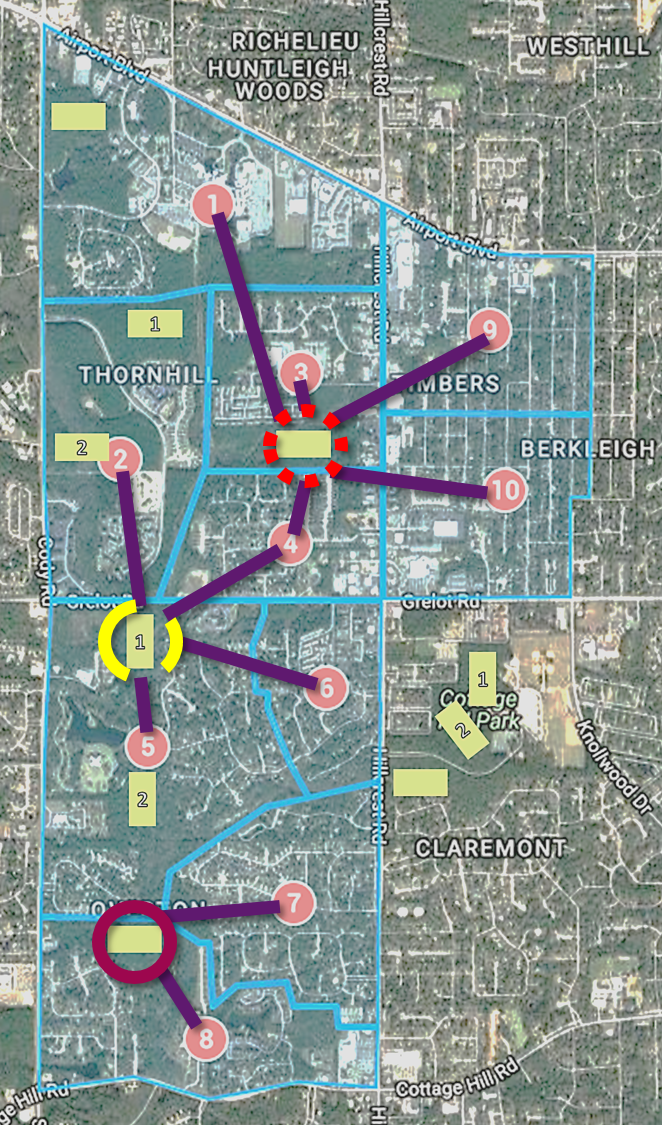
\includegraphics[width=0.35\textwidth]{d.png}
	\caption{Proposed CW network from Model D}
	\label{fig:networkd}
\end{figure}

The total cost of Model D is \$ 3.849 million, and the proposed number of CWs to be built is 3.

%\begin{table}[!h]
%	\caption{CW design options proposed from solving Model D.}
%	\label{table:resultscwd}
%	\centering
%	\makebox[\linewidth]{
%	\begin{tabular}{c c c c}
%		\csvautotabular{data/resultsd.csv}
%	\end{tabular}
%	}
%\end{table}

\subsection{Stochastic model: maximizing average success, Model S1}
%insert graphic

\subsection{Stochastic model: minimizing pollutant shortfall, Model S2}


\section{Computational study}
\subsubsection{Out-of-sample performance}
%model d s1 s2
%\begin{table}[!h]
%	\caption{Selected pollutants with the respective indicators coupled with average pollutant concentration in the wastewater source and the treatment targets.}
%	\label{table:polldata}
%	\centering
%	\makebox[\linewidth]{
%	\begin{tabular}{c c c c c}
%		\csvautotabular{data/pollutants.csv}
%	\end{tabular}
%	}
%\end{table}
%average success
%pollutant shortfall
\subsubsection{Increasing budget}
%how much can quality be improved by?

\section{Discussion}
%analysis

\section{Conclusion}

\subsection{Further Directions}
Proceeding from here, the next step would be to find a solution for the deterministic model, which will be done using MATLAB. After which, work will commence on developing the probabilistic model and running it. 


\clearpage

\section*{References}
\label{sec:references}
\addcontentsline{toc}{chapter}{\nameref{sec:references}}
\bibliography{mobile}
\clearpage

\section*{Appendix}
\label{section:appendix}
\addcontentsline{toc}{chapter}{\nameref{chap:appendix}}

\begin{table}[!h]
	\caption{Geographical information about the 14 blocks.}
	\label{table:geodata}
	\centering
	\begin{tabular}{c c c c c c}
		\csvautotabular{data/blockgeo.csv}
	\end{tabular}
\end{table}

\begin{table}[!h]
	\caption{Coordinates of the potential constructed wetlands sites.}
	\label{table:cwdata}
	\centering
	\begin{tabular}{ c c c }
		\csvautotabular{data/cwgeo.csv}
	\end{tabular}
\end{table}

\begin{table}[!h]
	\caption{Distance in $km$ between the wastewater sources and potential constructed wetlands sites.}
	\label{table:distdata}
	\centering
	\begin{tabular}{ c c c c c c c c c c c c}
		\csvautotabular{data/dist.csv}
	\end{tabular}
\end{table}

\begin{table}[!h]
	\caption{Selected pollutants with the respective indicators coupled with average pollutant concentration in the wastewater source and the treatment targets.}
	\label{table:polldata}
	\centering
	\makebox[\linewidth]{
	\begin{tabular}{c c c c c}
		\csvautotabular{data/pollutants.csv}
	\end{tabular}
	}
\end{table}

\begin{table}[!h]
	\caption{Construction cost of constructed wetlands with four different design options as well as projected area and flow capacity.}
	\label{table:ccwdata}
	\centering
	\begin{tabular}{c c c c}
		\csvautotabular{data/ccw.csv}
	\end{tabular}
\end{table}
\setcounter{equation}{0}
\renewcommand{\theequation}{A.\arabic{equation}}
\setcounter{figure}{0}
\renewcommand{\thefigure}{A.\arabic{figure}}
\setcounter{section}{0}
\renewcommand{\thesection}{A-\arabic{section}}
\newpage

\end{document}

